
\documentclass[a4paper,11pt]{article}
\usepackage[a4paper, margin=8em]{geometry}

% usa i pacchetti per la scrittura in italiano
\usepackage[french,italian]{babel}
\usepackage[T1]{fontenc}
\usepackage[utf8]{inputenc}
\frenchspacing 

% usa i pacchetti per la formattazione matematica
\usepackage{amsmath, amssymb, amsthm, amsfonts}

% usa altri pacchetti
\usepackage{gensymb}
\usepackage{hyperref}
\usepackage{standalone}

\usepackage{colortbl}

\usepackage{xstring}
\usepackage{karnaugh-map}

% imposta il titolo
\title{Electronics for Embedded Systems notes}
\author{Luca Seggiani}
\date{2026}

% spaziatura liste
\usepackage{enumitem}
\setlist[itemize]{noitemsep, topsep=4pt, partopsep=0pt, parsep=2pt, leftmargin=*}
\setlist[enumerate]{noitemsep, topsep=4pt, partopsep=0pt, parsep=2pt, leftmargin=*}

% imposta lo stile
% usa helvetica
\usepackage[scaled]{helvet}
% usa palatino
\usepackage{palatino}
% usa un font monospazio guardabile
\usepackage{lmodern}

\renewcommand{\rmdefault}{ppl}
\renewcommand{\sfdefault}{phv}
\renewcommand{\ttdefault}{lmtt}

% circuiti
\usepackage{circuitikz}
\usetikzlibrary{babel}

% testo cerchiato
\newcommand*\circled[1]{\tikz[baseline=(char.base)]{
            \node[shape=circle,draw,inner sep=2pt] (char) {#1};}}

% disponi il titolo
\makeatletter
\renewcommand{\maketitle} {
	\begin{center} 
		\begin{minipage}[t]{.8\textwidth}
			\textsf{\huge\bfseries \@title} 
		\end{minipage}%
		\begin{minipage}[t]{.2\textwidth}
			\raggedleft \vspace{-1.65em}
			\textsf{\small \@author} \vfill
			\textsf{\small \@date}
		\end{minipage}
		\par
	\end{center}

	\thispagestyle{empty}
	\pagestyle{fancy}
}
\makeatother

% disponi teoremi
\usepackage{tcolorbox}
\newtcolorbox[auto counter, number within=section]{theorem}[2][]{%
	colback=blue!10, 
	colframe=blue!40!black, 
	sharp corners=northwest,
	fonttitle=\sffamily\bfseries, 
	title=Theorem~\thetcbcounter: #2, 
	#1
}

% disponi definizioni
\newtcolorbox[auto counter, number within=section]{definition}[2][]{%
	colback=red!10,
	colframe=red!40!black,
	sharp corners=northwest,
	fonttitle=\sffamily\bfseries,
	title=Definition~\thetcbcounter: #2,
	#1
}

% disponi codice
\usepackage{listings}
\usepackage[table]{xcolor}

\definecolor{codegreen}{rgb}{0,0.6,0}
\definecolor{codegray}{rgb}{0.5,0.5,0.5}
\definecolor{codepurple}{rgb}{0.58,0,0.82}
\definecolor{backcolour}{rgb}{0.95,0.95,0.92}

\lstdefinestyle{codestyle}{
		backgroundcolor=\color{black!5}, 
		commentstyle=\color{codegreen},
		keywordstyle=\bfseries\color{magenta},
		numberstyle=\sffamily\tiny\color{black!60},
		stringstyle=\color{green!50!black},
		basicstyle=\ttfamily\footnotesize,
		breakatwhitespace=false,         
		breaklines=true,                 
		captionpos=b,                    
		keepspaces=true,                 
		numbers=left,                    
		numbersep=5pt,                  
		showspaces=false,                
		showstringspaces=false,
		showtabs=false,                  
		tabsize=2
}

\lstdefinestyle{shellstyle}{
		backgroundcolor=\color{black!5}, 
		basicstyle=\ttfamily\footnotesize\color{black}, 
		commentstyle=\color{black}, 
		keywordstyle=\color{black},
		numberstyle=\color{black!5},
		stringstyle=\color{black}, 
		showspaces=false,
		showstringspaces=false, 
		showtabs=false, 
		tabsize=2, 
		numbers=none, 
		breaklines=true
}

\lstdefinelanguage{x86}{ 
  keywords={AAA, AAD, AAM, AAS, ADC, ADCB, ADCW, ADCL, ADD, ADDB, ADDW, ADDL, AND, ANDB, ANDW, ANDL,
        ARPL, BOUND, BSF, BSFL, BSFW, BSR, BSRL, BSRW, BSWAP, BT, BTC, BTCB, BTCW, BTCL, BTR, 
        BTRB, BTRW, BTRL, BTS, BTSB, BTSW, BTSL, CALL, CBW, CDQ, CLC, CLD, CLI, CLTS, CMC, CMP,
        CMPB, CMPW, CMPL, CMPS, CMPSB, CMPSD, CMPSW, CMPXCHG, CMPXCHGB, CMPXCHGW, CMPXCHGL,
        CMPXCHG8B, CPUID, CWDE, DAA, DAS, DEC, DECB, DECW, DECL, DIV, DIVB, DIVW, DIVL, ENTER,
        HLT, IDIV, IDIVB, IDIVW, IDIVL, IMUL, IMULB, IMULW, IMULL, IN, INB, INW, INL, INC, INCB,
        INCW, INCL, INS, INSB, INSD, INSW, INT, INT3, INTO, INVD, INVLPG, IRET, IRETD, JA, JAE,
        JB, JBE, JC, JCXZ, JE, JECXZ, JG, JGE, JL, JLE, JMP, JNA, JNAE, JNB, JNBE, JNC, JNE, JNG,
        JNGE, JNL, JNLE, JNO, JNP, JNS, JNZ, JO, JP, JPE, JPO, JS, JZ, LAHF, LAR, LCALL, LDS,
        LEA, LEAVE, LES, LFS, LGDT, LGS, LIDT, LMSW, LOCK, LODSB, LODSD, LODSW, LOOP, LOOPE,
        LOOPNE, LSL, LSS, LTR, MOV, MOVB, MOVW, MOVL, MOVSB, MOVSD, MOVSW, MOVSX, MOVSXB,
        MOVSXW, MOVSXL, MOVZX, MOVZXB, MOVZXW, MOVZXL, MUL, MULB, MULW, MULL, NEG, NEGB, NEGW,
        NEGL, NOP, NOT, NOTB, NOTW, NOTL, OR, ORB, ORW, ORL, OUT, OUTB, OUTW, OUTL, OUTSB, OUTSD,
        OUTSW, POP, POPL, POPW, POPB, POPA, POPAD, POPF, POPFD, PUSH, PUSHL, PUSHW, PUSHB, PUSHA, 
        RCLL, RCR, RCRB, RCRW, RCRL, RDMSR, RDPMC, RDTSC, REP, REPE, REPNE, RET, ROL, ROLB, ROLW,
        ROLL, ROR, RORB, RORW, RORL, SAHF, SAL, SALB, SALW, SALL, SAR, SARB, SARW, SARL, SBB,
        SBBB, SBBW, SBBL, SCASB, SCASD, SCASW, SETA, SETAE, SETB, SETBE, SETC, SETE, SETG, SETGE,
        SETL, SETLE, SETNA, SETNAE, SETNB, SETNBE, SETNC, SETNE, SETNG, SETNGE, SETNL, SETNLE,
        SETNO, SETNP, SETNS, SETNZ, SETO, SETP, SETPE, SETPO, SETS, SETZ, SGDT, SHL, SHLB, SHLW,
        SHLL, SHLD, SHR, SHRB, SHRW, SHRL, SHRD, SIDT, SLDT, SMSW, STC, STD, STI, STOSB, STOSD,
        STOSW, STR, SUB, SUBB, SUBW, SUBL, TEST, TESTB, TESTW, TESTL, VERR, VERW, WAIT, WBINVD,
        XADD, XADDB, XADDW, XADDL, XCHG, XCHGB, XCHGW, XCHGL, XLAT, XLATB, XOR, XORB, XORW, XORL},
  keywordstyle=\color{blue}\bfseries,
  ndkeywordstyle=\color{darkgray}\bfseries,
  identifierstyle=\color{black},
  sensitive=false,
  comment=[l]{\#},
  morecomment=[s]{/*}{*/},
  commentstyle=\color{purple}\ttfamily,
  stringstyle=\color{red}\ttfamily,
  morestring=[b]',
  morestring=[b]"
}

\lstdefinelanguage{riscv}{
  keywords={
    LUI, AUIPC,
    JAL, JALR,
    BEQ, BNE, BLT, BGE, BLTU, BGEU,
    LB, LH, LW, LBU, LHU, LD,
    SB, SH, SW, SD,
    ADDI, SLTI, SLTIU, XORI, ORI, ANDI,
    SLLI, SRLI, SRAI,
    ADD, SUB, SLL, SLT, SLTU, XOR, SRL, SRA, OR, AND,
    ADDIW, SLLIW, SRLIW, SRAIW,
    ADDW, SUBW, SLLW, SRLW, SRAW,
    MUL, MULH, MULHSU, MULHU, DIV, DIVU, REM, REMU,
    MULW, DIVW, DIVUW, REMW, REMUW,
    LR.W, SC.W, AMOSWAP.W, AMOADD.W, AMOXOR.W,
    AMOAND.W, AMOOR.W, AMOMIN.W, AMOMAX.W,
    AMOMINU.W, AMOMAXU.W,
    LR.D, SC.D, AMOSWAP.D, AMOADD.D, AMOXOR.D,
    AMOAND.D, AMOOR.D, AMOMIN.D, AMOMAX.D,
    AMOMINU.D, AMOMAXU.D,
    FLW, FSW,
    FMADD.S, FMSUB.S, FNMSUB.S, FNMADD.S,
    FADD.S, FSUB.S, FMUL.S, FDIV.S, FSQRT.S,
    FSGNJ.S, FSGNJN.S, FSGNJX.S,
    FMIN.S, FMAX.S,
    FCVT.W.S, FCVT.WU.S, FCVT.S.W, FCVT.S.WU,
    FMV.X.W, FMV.W.X,
    FEQ.S, FLT.S, FLE.S,
    FLD, FSD,
    FMADD.D, FMSUB.D, FNMSUB.D, FNMADD.D,
    FADD.D, FSUB.D, FMUL.D, FDIV.D, FSQRT.D,
    FSGNJ.D, FSGNJN.D, FSGNJX.D,
    FMIN.D, FMAX.D,
    FCVT.W.D, FCVT.WU.D, FCVT.D.W, FCVT.D.WU,
    FCVT.S.D, FCVT.D.S,
    FMV.X.D, FMV.D.X,
    FEQ.D, FLT.D, FLE.D,
    CSRRW, CSRRS, CSRRC,
    CSRRWI, CSRRSI, CSRRCI,
    FENCE.I,
    FENCE,
    ECALL, EBREAK,
    MRET, SRET, URET,
    WFI,
    SFENCE.VMA,
    NOP, LI, LA, MV,
    NOT, NEG, NEGW,
    SEQZ, SNEZ, SLTZ, SGTZ,
    BEQZ, BNEZ, BLEZ, BGEZ, BLTZ, BGTZ,
    BGT, BLE, BGTU, BLEU,
    J, JR, RET,
    CALL, TAIL,
    RDINSTRET, RDCYCLE, RDTIME,
    CSRR, CSRW, CSRS, CSRC,
    CSRWI, CSRSI, CSRCI
  },
  keywordstyle=\color{blue}\bfseries,
  ndkeywordstyle=\color{darkgray}\bfseries,
  identifierstyle=\color{black},
  sensitive=false,
  comment=[l]{\#},
  morecomment=[s]{/*}{*/},
  commentstyle=\color{purple}\ttfamily,
  stringstyle=\color{red}\ttfamily,
  morestring=[b]',
  morestring=[b]"
}

\lstdefinelanguage{arm}{
  keywords={
    ADC, ADD, AND, BIC, CMN, CMP, EOR, MOV, MVN,
    RSB, RSC, SBC, SUB, TST, TEQ,
    MLA, MLS, MUL, SMLAL, SMULL, UMLAL, UMULL,
    QADD, QSUB, QDADD, QDSUB,
    QADD16, QADD8, QASX, QSAX,
    QSUB16, QSUB8, QSAX, QSUBADDX,
    ASR, LSL, LSR, ROR, RRX,
    B, BL, BX, BLX,
    BXJ,
    BEQ, BNE, BCS, BHS, BCC, BLO,
    BMI, BPL, BVS, BVC,
    BHI, BLS, BGE, BLT, BGT, BLE,
    BAL,
    LDR, LDRB, LDRH, LDRSB, LDRSH,
    LDRD, LDM, LDMIA, LDMIB, LDMDA, LDMDB,
    LDRT, LDRBT, LDRHT, LDRSBT, LDRSHT,
    STR, STRB, STRH, STRD,
    STM, STMIA, STMIB, STMDA, STMDB,
    STRT, STRBT, STRHT,
    PUSH, POP,
    SWP, SWPB,
    REV, REV16, REVSH,
    BFC, BFI, BFXIL, SBFX, UBFX,
    CLZ,
    LDREX, LDREXB, LDREXH, LDREXD,
    STREX, STREXB, STREXH, STREXD,
    DMB, DSB, ISB,
    MCR, MCRR, MRC, MRRC,
    MRS, MSR,
    CPS, SETEND, SVC, BKPT,
    CLREX, WFE, WFI, SEV,
    YIELD, NOP,
    VLDR, VSTR,
    VMOV, VABS, VNEG,
    VADD, VSUB, VMUL, VDIV,
    VMLA, VMLS, VNMLA, VNMLS, VNMUL,
    VMAX, VMIN,
    VSQRT,
    VCMP, VCMPE,
    VCVT,
    VCLZ, VCLS,
    VAND, VORR, VEOR, VBIC, VMVN,
    VLD1, VLD2, VLD3, VLD4,
    VST1, VST2, VST3, VST4,
    ADR, ADCS, ADDS, SUBS, MOVS, ANDS, ORRS, EORS
  },
  keywordstyle=\color{blue}\bfseries,
  ndkeywordstyle=\color{darkgray}\bfseries,
  identifierstyle=\color{black},
  sensitive=false,
  comment=[l]{@},
  morecomment=[l]{;},
  morecomment=[s]{/*}{*/},
  commentstyle=\color{purple}\ttfamily,
  stringstyle=\color{red}\ttfamily,
  morestring=[b]',
  morestring=[b]"
}

\lstset{style=codestyle, language=C}

% disponi sezioni
\usepackage{titlesec}

\titleformat{\section}
	{\sffamily\Large\bfseries} 
	{\thesection}{1em}{} 
\titleformat{\subsection}
	{\sffamily\large\bfseries}   
	{\thesubsection}{1em}{} 
\titleformat{\subsubsection}
	{\sffamily\normalsize\bfseries} 
	{\thesubsubsection}{1em}{}

% tikz
\usepackage{tikz}

% float
\usepackage{float}

% grafici
\usepackage{pgfplots}
\pgfplotsset{width=10cm,compat=1.9}

% disponi alberi
\usepackage{forest}

\forestset{
	rectstyle/.style={
		for tree={rectangle,draw,font=\large\sffamily}
	},
	roundstyle/.style={
		for tree={circle,draw,font=\large}
	}
}

% disponi algoritmi
\usepackage{algorithm}
\usepackage{algorithmic}
\makeatletter
\renewcommand{\ALG@name}{Algorithm}
\makeatother

% disponi numeri di pagina
\usepackage{fancyhdr}
\fancyhf{} 
\fancyfoot[L]{\sffamily{\thepage}}

\makeatletter
\fancyhead[L]{\raisebox{1ex}[0pt][0pt]{\sffamily{\@title \ \@date}}} 
\fancyhead[R]{\raisebox{1ex}[0pt][0pt]{\sffamily{\@author}}}
\makeatother

\begin{document}
% sezione (data)
\section{Lesson 12-10-26}

% stili pagina
\thispagestyle{empty}
\pagestyle{fancy}

% testo

In the last lesson we introduced programmable memories, covering:
\begin{itemize}
	\item \textbf{MPROM}s (\textit{Mask Programmable ROMs}), programmable only once by altering the design at production time;
	\item \textbf{OTP-ROM}s (\textit{One Time Programmable ROMs}), based on fixed MOSFET paths programmed only once by \textit{blowing fuses};
	\item \textbf{EPROM}s (\textit{Erasable Programmable ROMs}), programmable electrically, and erasable only via photoelectric effects (shining a light on them). These were based on \textbf{FAMOS} (\textit{Floating gate Avalanche MOS}) transistors;
	\item \textbf{EEPROM}s (\textit{Electrically Erasable Programmable ROMs}), programmable and erasable electrically. These were based on \textbf{FLOTOX} (\textit{FLoating gate Tunneling OXide MOS}) transistors.
\end{itemize}

\subsection{Flash memory}

We now cover \textbf{flash} memory storage, which seeks to lower the cost and latency problem of common EEPROM memory, while still providing a completely electric read/write interface.

\subsubsection{NOR Flash}

\textbf{NOR Flash} memory is based on FLOTOX transistors with thin layers on the source side of the channel.

\begin{center}
	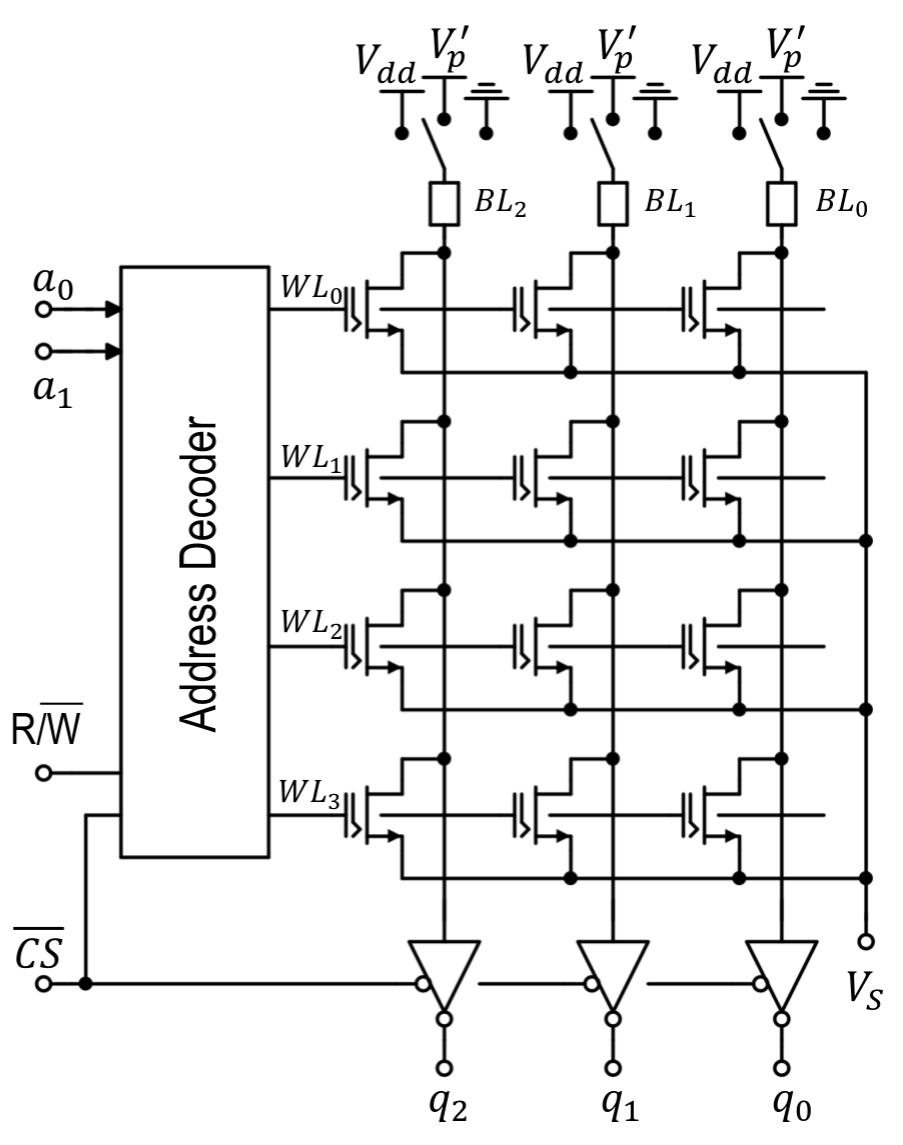
\includegraphics[scale=0.22]{../figures/nor_flash.png}
\end{center}

All Sources are tied together and not connected to ground.
All FLOTOX transistors are not programmed after fabrication, so that they behave normally and the initial content of the memory is all 1s.

NOR Flash transistors are programmed and erased in different ways:
\begin{itemize}
	\item \textbf{Hot Electron Programming} is used for \textit{programming}, to avoid affecting other transistors;
	\item \textbf{Tunneling effect} is used for erasing.
\end{itemize}

Let's see in detail:

\begin{itemize}
	\item To \textbf{program} the memory, the word is selected via its address and data is provided on the data bus.

	      The select word line (targeting the gates) is driven at programming voltage $V_p$, and all other word lines are kept at ground.

	      The selected bit lines (targeting the drains) are also driven at programming voltage $V_p'$, and all other bit lines are kept at ground.

	      Lastly, sources are connected to ground with $V_S = 0 \, \mathrm{V}$.

	      The high energy electrons which end up traveling through the channel are thus able to be injected in the gate, raising the gate threshold $V_{TH}$ and encoding a logic 0;

	\item To perform a \textbf{full erase} of the memory, all word lines and bit lines are grounded.

	      The source is then driven to high programming voltage.

	      Since the thin oxide layer is on the source side, the result is that we experience electron tunneling from gate to source, and a logic 1 is encoded in every transistor (so each memory location).

	\item A \textbf{block erase} is also possible by splitting the $V_S$ line among different groups of transistors (at least as big as a single word).
	      Usually block size ranges from a few Kbytes to hundreds of Kbytes.

	      Sources of different blocks can be independently driven: the erase is therefore applied to only one block at a time.
\end{itemize}

\subsubsection{NOR Flash peformance}

In regards to performance, we have that the \textbf{read} operation is identical to Mask Programmable ROM, OTP-ROM, EPROM and EEPROM.
The performance in \textbf{writing}, other hand, sacrifices single bit access while erasing (present on EEPROMs). When writing, an entire block is erased and rewritten, even when writing a single word.

This calls for more complex memory writing mechanisms, which need temporary buffers to store the blocks being modified.
One such mechanism is detailing in the figure.
\begin{center}
	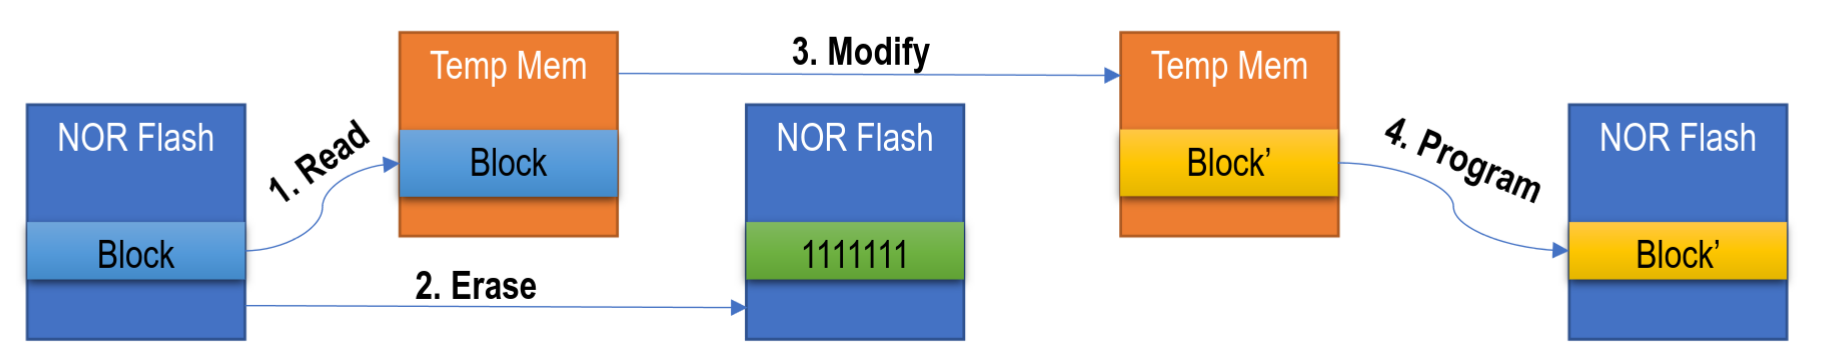
\includegraphics[scale=0.22]{../figures/nor_op.png}
\end{center}

Lastly, we note that for NOR Flash memory a \textbf{CFI} (\textit{Common Flash memory Interface}) exists, and is agreed upon and used by constructors.
\begin{itemize}
	\item
	      Reading is performed as in a ROM;
	\item
	      Writing is based on commands: a standard set exists, and software drivers are usually used to access these kinds of memories.
\end{itemize}

\subsubsection{NAND Flash}

\textbf{NAND Flash} is the NAND version of NOR flash.
It still uses FLOTOX transistors, but with thin oxide on the drain side.
The difference is that tunneling is used for both \textit{reading} and \textit{writing} cells.

\begin{center}
	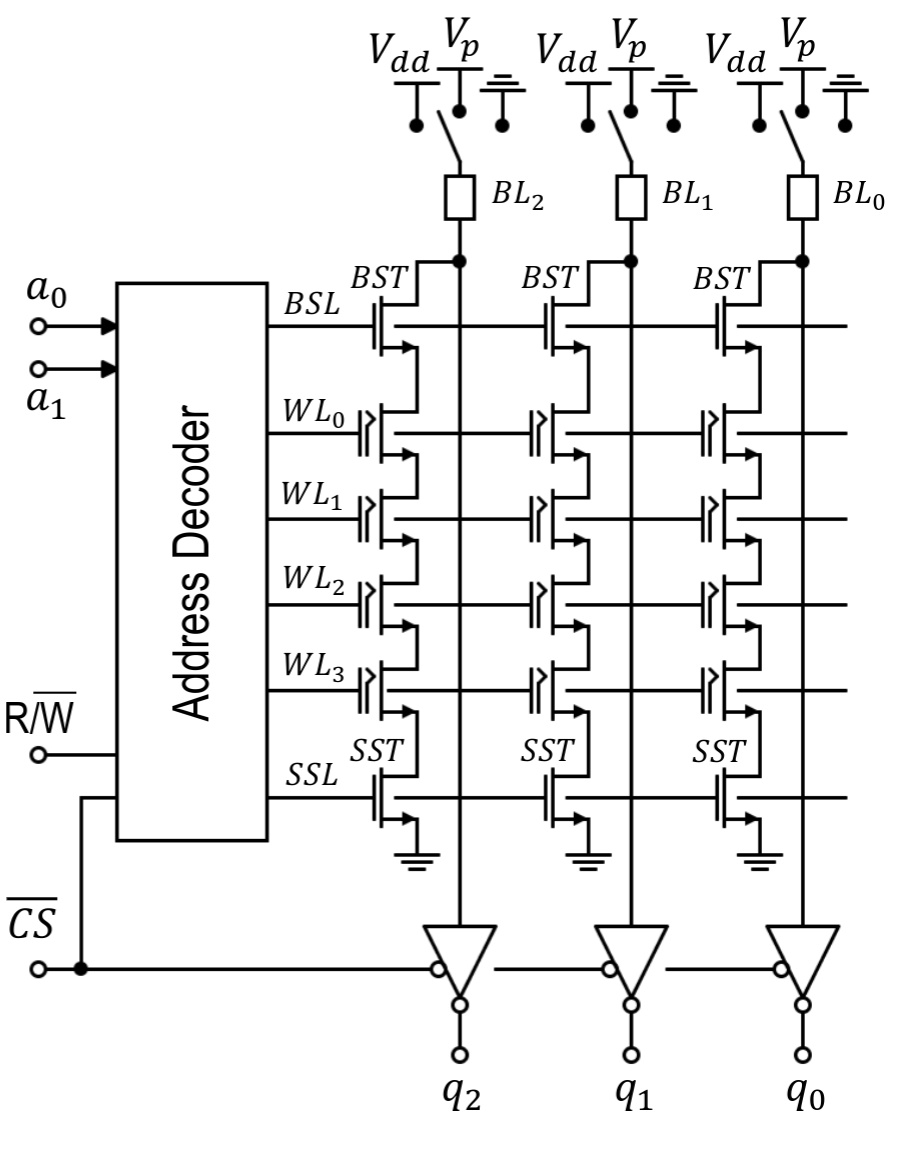
\includegraphics[scale=0.22]{../figures/nand_flash.png}
\end{center}

As with MPROMs (see lesson 7), NAND topology is slower (higher parasitic capacitances and resistances), but denser (lower costs and size).

To enable correct usage, access transistors are placed at the top and bottom of a series:
\begin{itemize}
	\item At the top (drain side) we have a \textbf{BST} (\textit{Bit Line Select Transistor});
	\item At the bottom (source side) we have a \textbf{SST} (\textit{Source Select Transistor}).
\end{itemize}

All FLOTOX transistors are not programmed after fabrication, so the initial content of the memory are all 1s.

In NAND Flash, all gate voltages are complemented compared to NOR topology.
Voltage values used in NAND Flash memories are:
\begin{itemize}
	\item $V_{th}$ is the nominal threshold voltage of a non programmed transistor;
	\item $V_{thprog}$ is the threshold voltage of a programmed transistor;
	\item $V_{pass} > V_{thprog}$ is a gate voltage such that all transistors are conducting, regardless of their programming state;
	\item $V_{read}$ is a gate voltage such that only non programmed transistors are conducting;
	\item $V_{off} < V_{th}$ is a gate voltage such that all transistors are not conducting.
\end{itemize}

We move on to operations.
\begin{itemize}
	\item First off, \textbf{reading} is non trivial. We first set all bit lines to $V_{dd}$ (so that the pull-up transistors actually pull up).

	      Then we set the selected word line to $V_{read}$, and all others to $V_{pass}$.
	      This means that all transistors, except in the word to be read, are conducting.

	      At this point:
	      \begin{itemize}
		      \item If the transistor in the word is not programmed, it is conducting: the Bit Line is grounded, and the output is logic 1;
		      \item If the transistor in the word is programmed, it is not conducting: the series is interrupted, the Bit Line remains high, and the output is logic 0.
	      \end{itemize}

	      Note that reading a NAND flash memory is slow, as the NAND topology has much higher delays than the NOR topology.
	      For this reason the memory is divided in \textbf{blocks}: each block is tens or hundreds of Kbytes. Each block is divided in \textbf{pages}, where ach page is tens or hundreds of bytes. A page is a row, or a fraction of a row, of the bit cell array.

	      Most NAND Flash Memories are read \textit{page by page}, storing in a temporary SRAM buffers. Words are read sequentially within a page, and no random access to individual words is permitted.
	      Because of this, NAND Flash Memory is not a drop-in replacement of a ROM: it cannot be used to store and execute code directly.

	\item \textbf{Programming} a transistor iw performed by setting the selected word line to $V_p$, and all the other word lines to $V_{pass}$.

	      Then, the desired bit line is set to ground, and all the other bit lines to $V_p$.

	      Lasly, the BSTs are enabled and the SSTs disabled, meaning the sources are floating (Which is the programming condition for FLOTOX transistors via electron tunneling).

	      With this method we do program the selected transistors, and other transistors aren't affected:
	      \begin{itemize}
		      \item Transistors in other words (row) have a small $V_{GD}$;
		      \item Other transistors in the same word have $V_{GD} = 0 \, \mathrm{V}$
	      \end{itemize}

	\item \textbf{Erasing} is done in blocks.

	      BST and SST access transistors are deactivated, so that all channels are left floating.

	      Then all word lines are grounded.

	      The erasure tunneling happens directly via the \textit{substrate}, which is set to progamming voltage $V_p$.

	      This means we erase an entire \textit{block}, or the entire memory.
	      For this reason, blocks are in isolated substrate wells.
	      All blocks can be erased concurrently, affecting the entire memory.
\end{itemize}

\subsubsection{NAND Flash performance}

We already said that NAND Flash provides very low read efficency, and as such is more suited to whole page caching, with serial access protocols.

The serial interface is similar to \textbf{SPI}, with up to 4 parallel bits (non-SPI mode).

To summarize, to increase performance a page is first transferred to an
internal cache (made up of SRAM).
Reads and writes always occur from/to the cache, with the internal memory controller governing read/writes to and from the actual NAND memory cells.

As with NOR Flash, the protocol defines a number of commands.

Lastly, we note that we need to read – modify – rewrite, like in the NOR Flash Memory case.
It’s easier to write the updated block to an empty block, marking the initial one for erasing.

\subsection{Summary of ROM memories}

We show graph of Write Ability and Storage Permanence of ROM memories (see section 6.0.2).

\begin{center}
	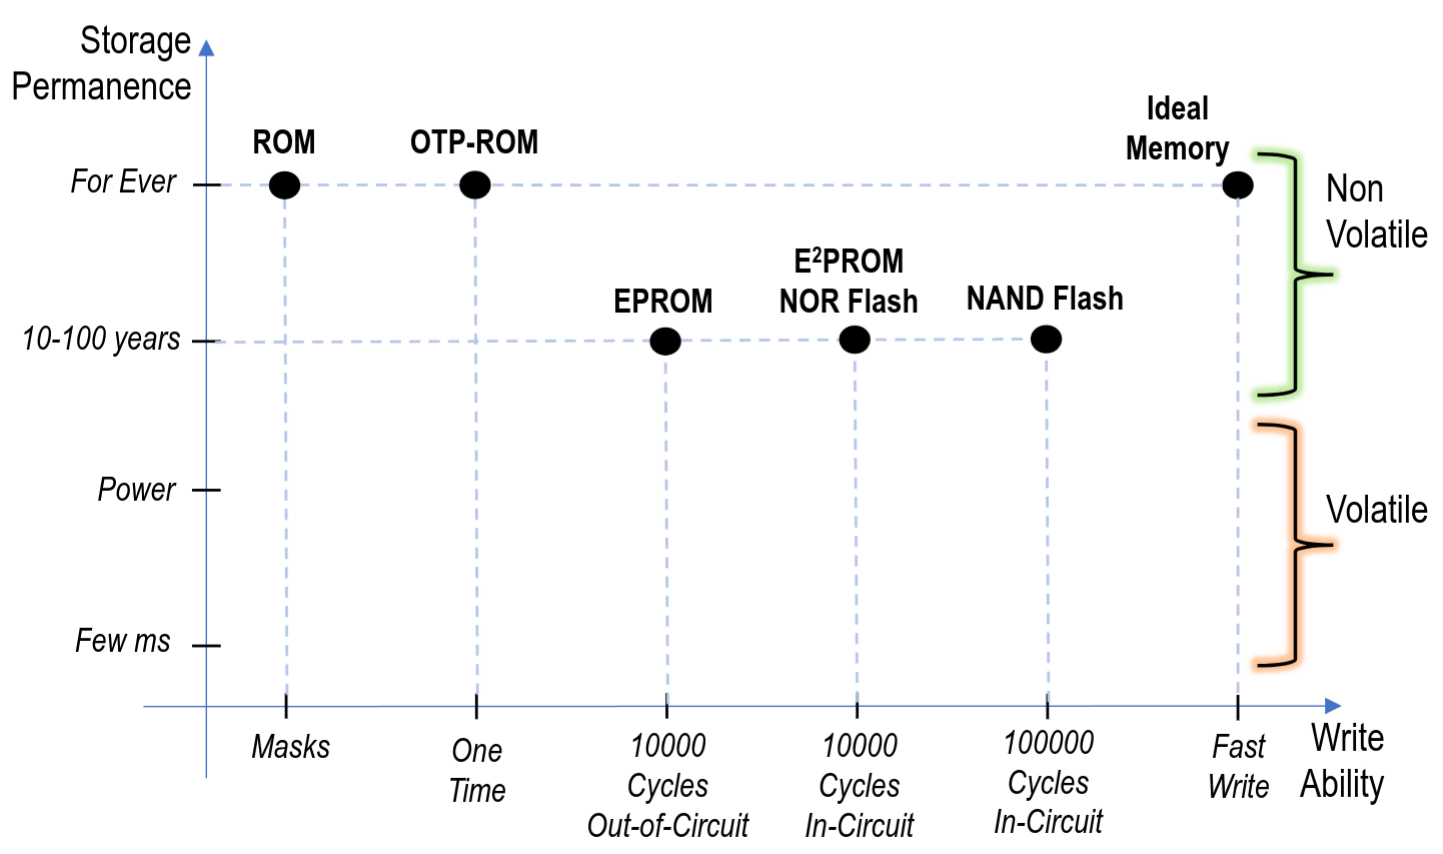
\includegraphics[scale=0.22]{../figures/rom_comp.png}
\end{center}

We see that:
\begin{itemize}
	\item All ROM memories have a large penalty in writing, and as such are used mostly to read data;
	\item Flash memories are faster (than for instance EEPROMs), but erasing and writing not at word level;
	\item All ROM memories are \textit{non volatile}, but this is sometimes not necessary.
	      In these cases we can sacrifice storage permanence by write as fast as reading, using word and bit levels (instead of programming voltages).
	      With this method we can use standard access methods, with no need of programming and erasing.


\end{itemize}

\subsection{Read Only Memories}

We now move on to \textbf{RAM}s (\textit{Read Only Memories}).
RAM denotes memories that are fast to write, and random access.
ROMs are also random access, but RAMs are much faster than E2PROMs and Flash memories (several order of magnitude faster especially in writing).

RAMs usually allow single bit and single word access in reading and writing, with no distinction between programming and erasing: write is identical in the two cases (0 $\rightarrow$ 1 and 1 $\rightarrow$ 0).

There are two main kind of RAMs:
\begin{itemize}
	\item \textit{Static} RAM (\textbf{SRAM}, \textbf{CAM} or \textit{Content Addressable Memory});
	\item \textit{Dynamic} RAM (\textbf{DRAM}, \textbf{SDRAM}, \textbf{DDR}).
\end{itemize}

\subsubsection{Static RAM}

Static RAM relies on \textit{bistable} circuits, that is the usual sequential data latches.

As we saw in 3.2, a NOT loop is a basic example of a bistable circuit, with an unstable center state.
\begin{center}
	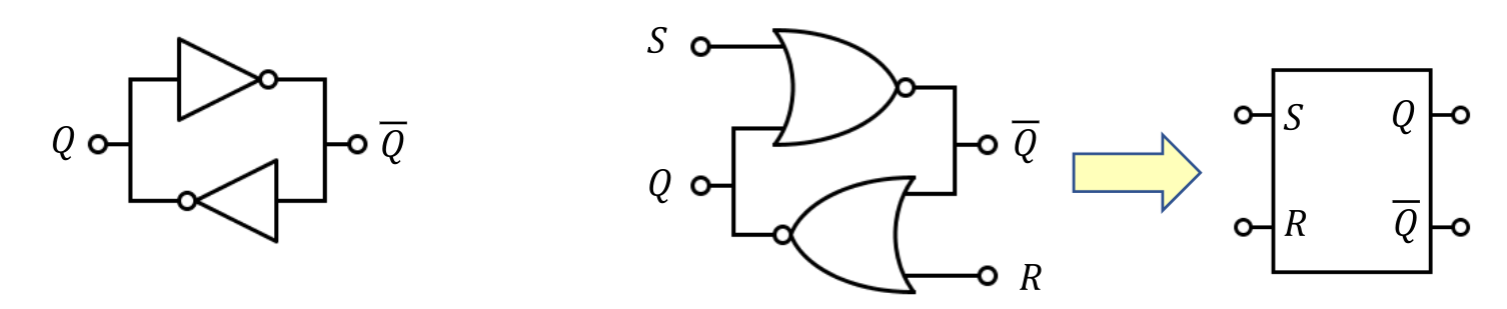
\includegraphics[scale=0.22]{../figures/sr_latch.png}
\end{center}

To create an SRAM cell from an SR latch, we need a special topology.
\begin{center}
	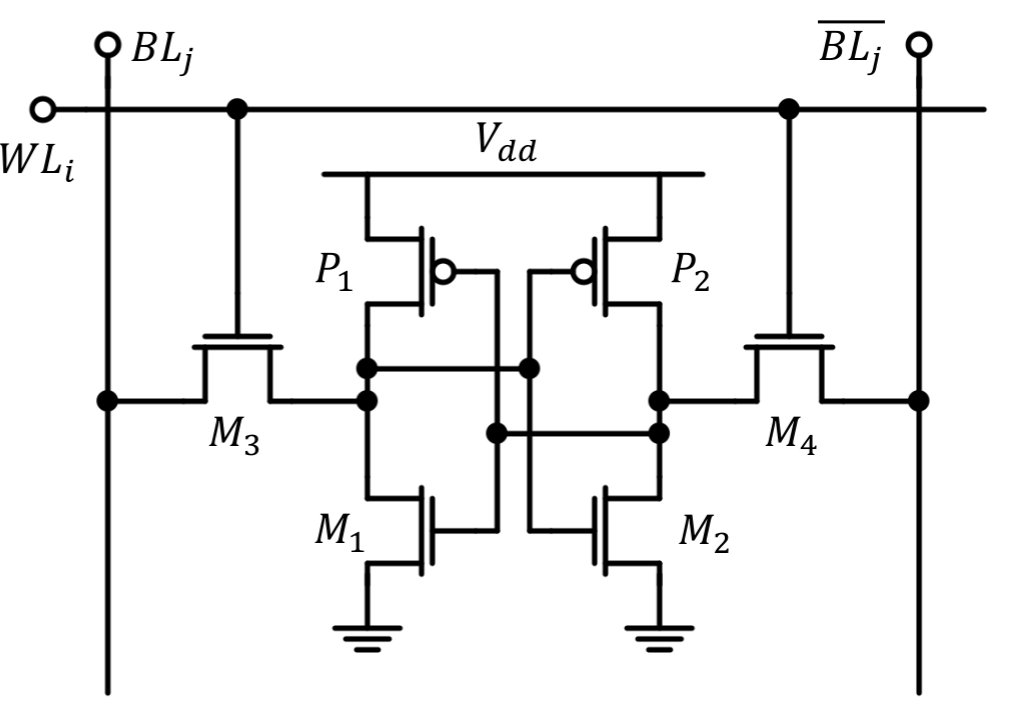
\includegraphics[scale=0.22]{../figures/sram_cell.png}
\end{center}

This features:
\begin{itemize}
	\item The $M_1$, $M_2$, $P_1$ and $P_2$ transistors to realize the basic bistable cell;
	\item The \textit{access} transistors $M_3$ and $M_4$, configured as pass transistors. These allow programming of the bit.
\end{itemize}

We note the two Bit Lines for each bit cell: one affirmed and one complemented.
A single Word Line, on the other hand, drives the gates of both the access transistors, enabling reads/writes to the bistable cell.

\par\smallskip

Let's now look at the organization of static RAM cells to form a full SRAM:

\begin{center}
	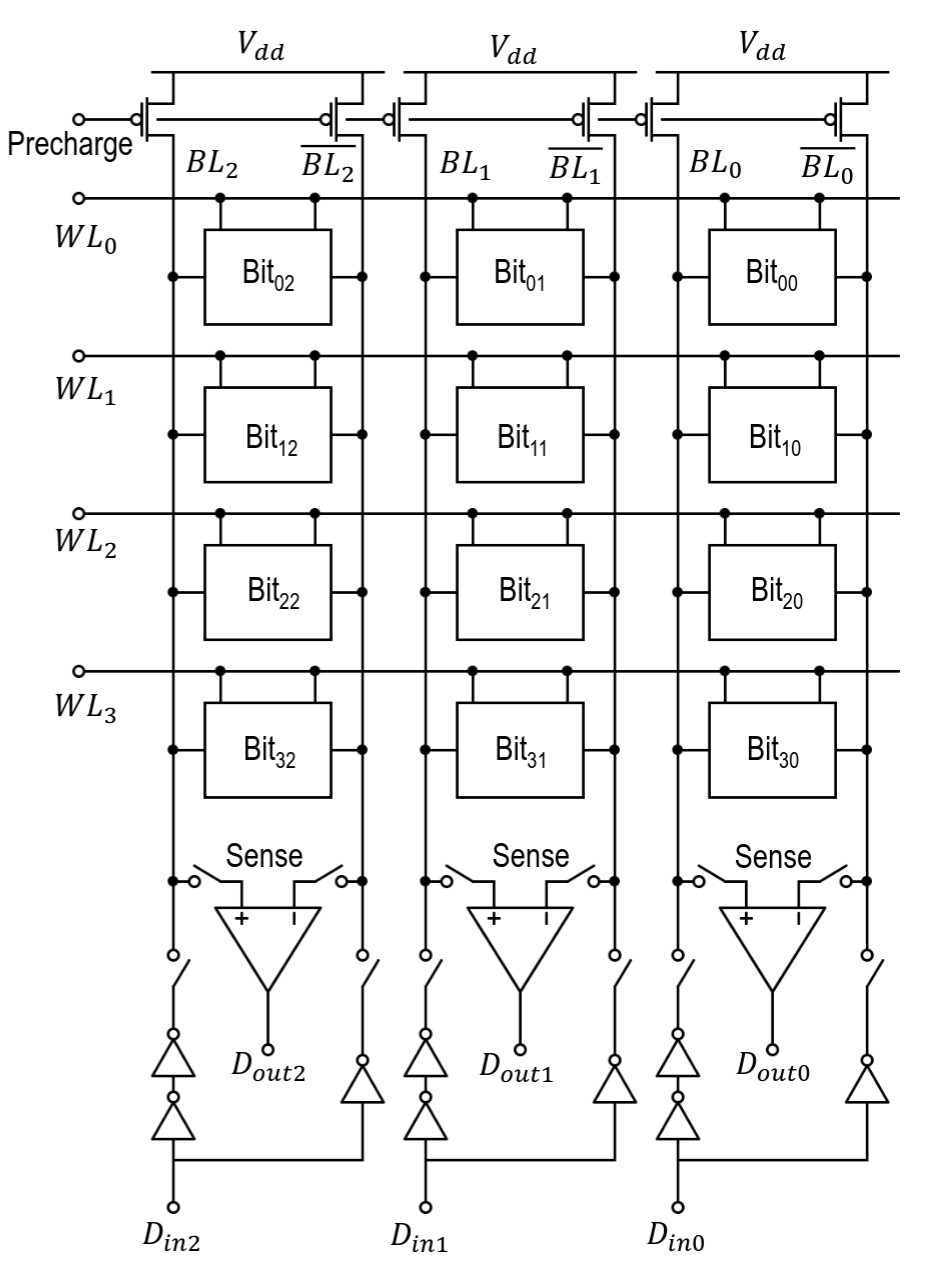
\includegraphics[scale=0.28]{../figures/sram_topo.png}
\end{center}

We see that a number of components have to be studied:
\begin{itemize}
	\item The single \textit{bit cell} is the same as we already saw. Note that a single pair of affirmed and complemented bit lines is shared across multiple cells;
	\item The \textit{precharge} circuit. This is used to precharge the bitlines to a level which won't interact with the values stored in the bit cells on reads;
	\item The \textit{sense amplifier}: this is used to sense values in the bit lines and amplify them to full logic levels. All of this machinery is really needed because sharing multiple bit lines across bit cells multiplies the resistances and capacitance experienced by these;
	\item Lastly we need a \textit{column decoder} and \textit{mux} for allow I/O data lines at the bit lines.
\end{itemize}

Let's now go through \textit{operations}.
\begin{itemize}
	\item \textbf{Reading}. This happens in a few steps.

	      \begin{enumerate}
		      \item First we charge both the bitlines to $V_{dd}$. Then we detach the precharge source. This means that the $V_{dd}$ voltage is mantained through wire capacitance on the bit lines (usually in the order of picofarads);
		      \item After the bitlines are left floating, the $M_3$ and $M_4$ passgates are opened. This means that one side (the high side) of the bit lines will stay high, and the other will go low. By sensing the voltage difference across them, we can recover the data which was initially stored in the bit line.
	      \end{enumerate}

	      Note that in this operation $M_3$ starts conducting current, thus raising the voltage at $M_2$'s gate. To avoid bit flips, $M_3$ should be sized smaller than $M_1$ (to have a higher $R_{DSon}$ resistance and take more voltage in the voltage divider that is formed).

	\item \textbf{Writing}. This is arguably simpler.

	      \begin{enumerate}
		      \item We first load the bit lines (affirmed and complemented) to respectively the affirmation and the complement of the value we want to store. This process is similar to precharging, with the difference that the voltage applied to the bit lines is kept until wire capacitance charge, and throughout the whole writing process (so the bit cells are actively driven);
		      \item To actively drive the bit cells we then just raise the word line, so that the bitline values propagate to the bit cell.
	      \end{enumerate}

	      Note that for this operation to work we need to be able to force a bit flip, and thus the pass gate transistors $M_3$ and $M_4$ should be larger than the PMOS transistors $P_1$ and $P_2$ (so that their side in the voltage divider is larger).
\end{itemize}

\subsubsection{SRAM performance}

SRAM performance is great in both reading and writing.

\begin{itemize}
	\item For the \textit{read operation} we said that the low side nMOS transistors in the bistable circuit should be larger than the corresponding nMOS access transistors.
	      This means that the ON resistance is lower for the low side nMOS transistors.

	      We then have that the sense amplifier detects very small changes of the input voltages, with $\Delta V$ in the order of a few hundred millivolts.

	      As such, the performance of reading is very fast, ranging from a few nanoseconds to tens of nanoseconds;

	\item For the \textit{write operation} we said that the nMOS access transistors should be larger than the high side pMOS transistors in the bistable circuit.
	      Sometimes the pMOS are implemented using resistances, or pMOS that are always conducting, designed to have a high $R_{DSon}$.
	      The exact ratio of all transistors depends on technological parameters: transistors are not minimum size.

	      The performance for writing is very fast, ranging from a few nanoseconds to tens of nanoseconds, which is comparable to the read operation.

	      There are also \textit{no limits} in the number of write operations (far different from most ROMs we saw), and \textit{no distinction} between writing 0 or 1.
\end{itemize}

\subsubsection{SRAM variants}

A few variations on SRAM are available.
\begin{itemize}
	\item \textbf{NVRAM} (\textit{Non Volatile RAM}): a battery keeps power for several years. It is more expensive, larger in physical size, and heavier;
	\item \textbf{Multiport SRAM}: features independent ports with separate busses, independent access transistors and row and column circuits.

	      This allows multiple users to read concurrently at multiple location (even the same one).
	      They can also read a location while writing another location.

	      Note that, when reading a location while writing the same location, the result of reading is not defined.

	      Users can also write multiple different locations concurrently, but still note that writing the same location from different ports yields an undefined stored value.
\end{itemize}

\subsection{Dynamic RAM}

Our goal with dynamic RAM is to design a much smaller bit cell, to make a fast and cheap memory.

The idea is to store information as charge on a capacitor: a capacitor is a form of analog memory where if charge is present, the logic value is 1; if charge is not present, the logic value is 0.

Lastly, note that the capacity used in DRAM is actually the parasitic capacitance $C_{bit}$ of a special transistor.
A second \textit{access} transistor allows to charge or observe the storage capacity $C_{bit}$.

\begin{center}
	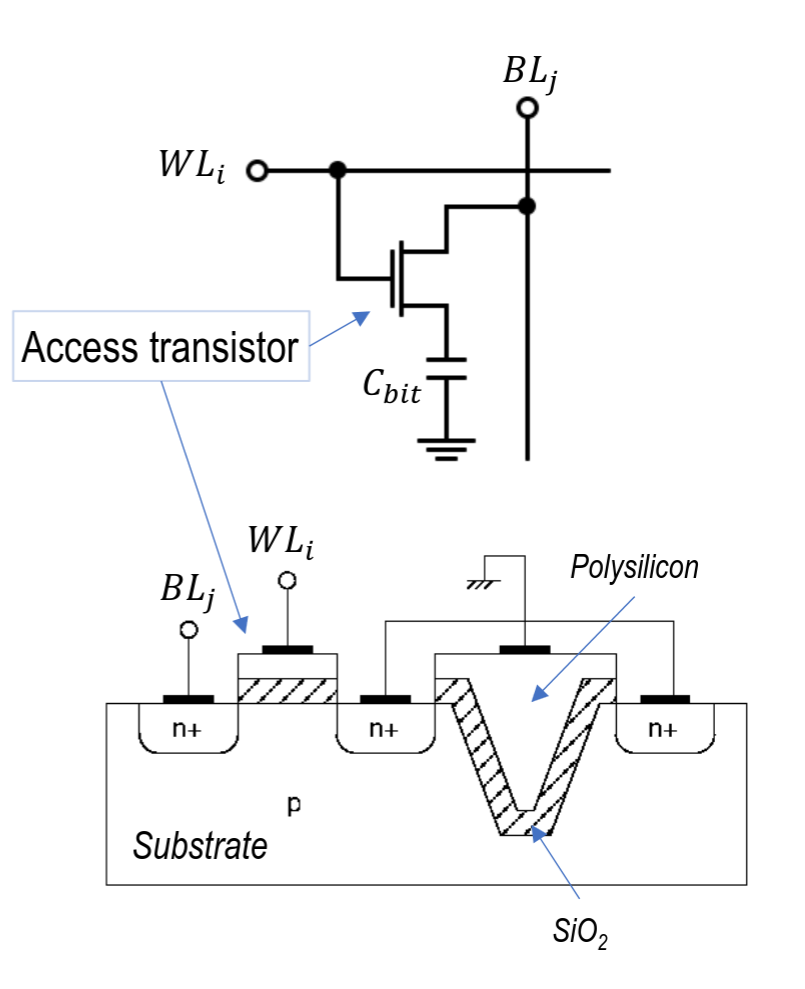
\includegraphics[scale=0.22]{../figures/dram_cell.png}
\end{center}

Looking at the layout cross-section, the nMOS access transistor is a standard one.
Te capacity transistor, however, is a so-called \textbf{trench capacitor}, comprised of an nMOS transistor with Source and Drain connected together.
These are in turn onnected to the Source of the access transistor.
The polysilicon Gate goes inside the substrate, increasing the area $A$ of the gate.
The gate is connected to ground, so that the equivalent capacitance is:
$$
	C_{bit} = C_{ox} \cdot A
$$

To improve the analog memory, $C_{bit}$ should be the highest possible.
Technology is defined to increase the parasitic capacitance: it cannot be embedded on the same integrated circuit as standard logic.

The DRAM bit cell is small, much smaller than SRAM.
\textit{Stacked capacitors} then allow for smaller footprint in planar technology.
This allows DRAM memory to be far cheaper than SRAM.

Of course, there are problems associated with DRAM:
\begin{itemize}
	\item
	      Leakage currents destroy the information after some time (milliseconds), so we need to periodically refresh the data stored;
	\item
	      Reading the charge on the capacitor requires to remove some charges, which need to be restored after reading to not lose data.
\end{itemize}

Let us now look at the usual DRAM topology.

\begin{center}
	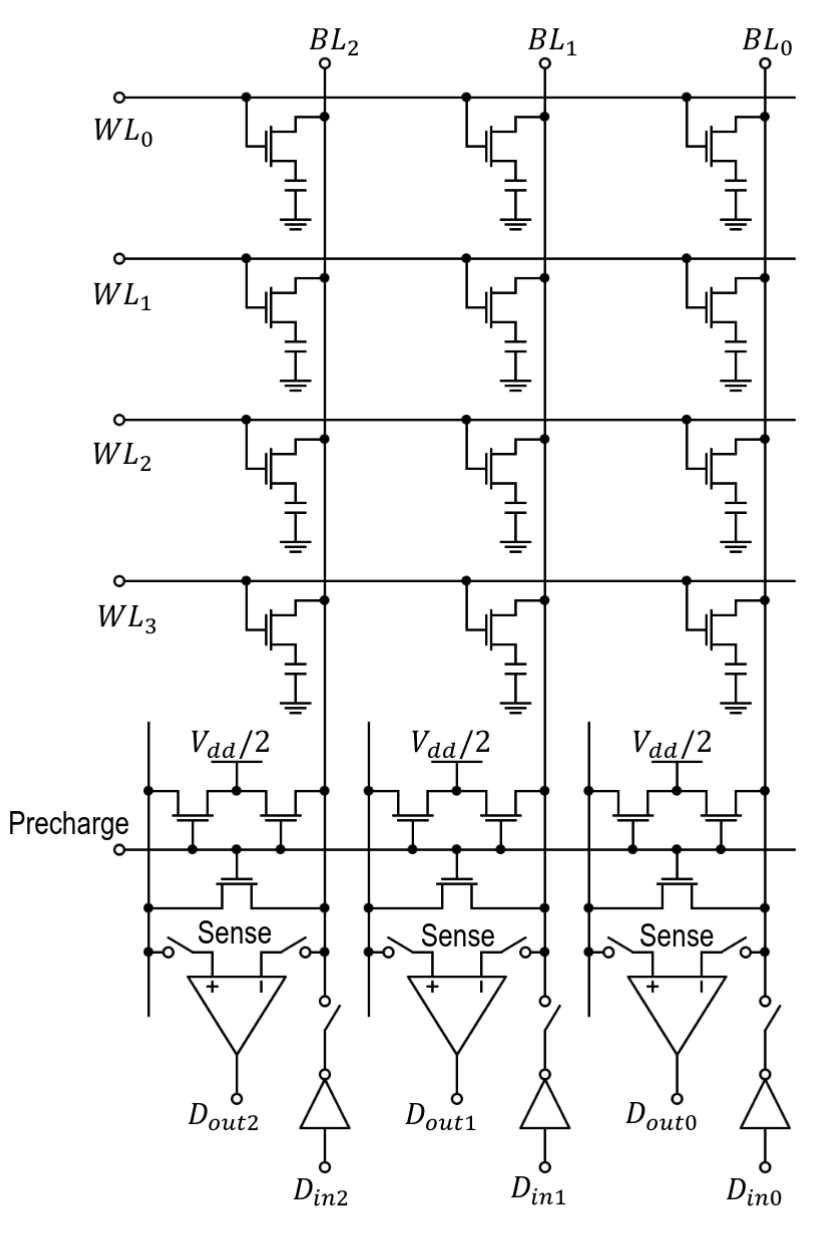
\includegraphics[scale=0.28]{../figures/dram_topo.png}
\end{center}

We see:
\begin{itemize}
	\item The usual matrix of bit cells, organized in word lines and bit lines. The capacity is easy to connect in this configuration as the word line just drives the access transistor gate, and the capacity drives the bit line (through the access transistor's source);
	\item We the have the \textit{precharge} circuit to connect bit lines to $\frac{V_{dd}}{2}$. This is a nice unbiased voltage we can use to extract useful $\Delta V$ from the capacities;
	\item We then have the \textit{sense amplifier}. It is a differential amplifier to detect small voltage differences. To have a $\Delta V$ difference in the first place, we need an additional comparison line. This is usually the $\frac{V_{dd}}{2}$ line from before;
	\item As with SRAM, we have the \textit{I/O} section with inputs and outputs, switches driven by column decoder and mux.
\end{itemize}

Let's see the \textit{operations}:
\begin{itemize}
	\item For \textbf{reading}, we start with all wordlines inactive, and precharge the bitlines to $\frac{V_{dd}}{2}$.

	      We then activate the selected wordline.
	      Charge is thus shared between the $C_{bit}$ capacitances and $C_L$, which is the cunulative capacitance of a bit line.

	      When we then activate the sense amplifiers and select the desired word, the sense amplifiers detects the small change, positive or negative. This gets us the final read result.

	      Note that the final voltage on the storage capacitor is close to $V_{ref}$ (our $\frac{V_{dd}}{2}$): information is lost (we say that reading is \textit{destructive}).
	      To restore it we need to write after reading.
	      This is performed internally by the memory, so it is not necessary to issue a write command.
	      On the other hand, rewriting is necessary also in other words of the same row (even if not read).

	      We can do some calculations to evaluate the charge transfer between $C_{bit}$ and $C_L$ in both the reading 1 and reading 0 state:
	      \begin{itemize}
		      \item For the 1 state, we start by computing the total charge on the $C_{bit}$ capacity and the $C_L$ capacity before raising the word line. Assuming that after raising the word lines these are equalized, we have to find the resulting voltage. In symbols:
		            $$
			            \begin{cases}
				            Q_{tot}'  & = C_{bit} (V_{dd} - V_{th}) + C_L V_{ref} \\
				            Q_{tot}'' & = (C_{bit} + C_L) V_X
			            \end{cases}
			            \implies
			            V_X = \frac{C_{bit} (V_{dd} - V_{th}) + C_L V_{ref}}{C_{bit} + C_L}
		            $$
		            At this point we compute the final $\Delta V$ as the difference between the resulting $V_X$ and the $V_{ref}$ the sensing amplifiers compare against:
		            $$
			            \Delta V = V_X - V_{ref} = \frac{C_{bit}}{C_{bit} + C_L} \left( V_{dd} - V_{th} + V_{ref} \right)
		            $$
		            Lastly, note that $V_{ref} \approx \frac{V_{dd}}{2}$ as per previous discussions, so we can say;
		            $$
			            \Delta V = \frac{C_{bit}}{C_{bit} + C_L} \left( \frac{V_{dd}}{2} - V_{th} \right)
		            $$

		      \item For the 0 state, we do the same thing in reverse. Assume the $C_{bit}$ capacity starts low, with zero charge:
		            $$
			            \begin{cases}
				            Q_{tot}'  & = 0 + C_L V_{ref}     \\
				            Q_{tot}'' & = V_X (C_{bit} + C_L)
			            \end{cases}
			            \implies
			            V_X = \frac{C_L}{C_{bit} + C_L} V_{ref}
		            $$
		            We compute the final $\Delta V$ the same as before:
		            $$
			            \Delta V = - \frac{C_{bit}}{C_{bit} + C_L} V_{ref} = - \frac{C_{bit}}{C_{bit} + C_L} \frac{V_{dd}}{2}
		            $$
		            using the same value of $V_{ref}$ as before.
	      \end{itemize}

	      What we wanted to show is that $\Delta V_1 \approx - \Delta V_2$, so that the sensing amplifiers see basically the same voltage delta in both reading cases.

	      At this point we just have to note that at the end of the read operation the voltage on the storage capacitor is $V_X$, which is very close to $V_{ref}$.
	      The original logic value is lost, and in fact all bits in the same row are lost, even if they are not part of the word that is being read.
	      Still, the information is known at the output of the sense amplifiers!
	      This is true for all columns, even those that were not selected: the logic value can thus be written back by driving the Bit Line with an appropriate voltage (we'll see write shortly), and the original logic value is restored on $C_{bit}$.
	      This also applies to all bits in the row, as the value is taken from the sense amplifier of the corresponding column.

	\item For \textbf{writing}, we also start with all wordlines inactive.

	      We then apply the desired to the bit lines, and precharge the bit lines of all other words to $V_{ref}$ (as to not interfere with their values once we raise the word line).

	      After this setup we raise the word line, and storage capacitors are charged or discharged to the wanted values.

	      Note that this seems fast, but has the same destructive effect on bits we are not interested in as reading: we require a read (through the sense amplifiers) and a write back.
	      This means that the performance is the same as reading.

\end{itemize}

A solution for DRAM memory is the \textit{Comparison Line}.
The sense amplifier is placed in the middle of a Bit Line: the other half of the Bit Line used for comparison.

When \textit{precharging}, both halves of the Bit Line are precharged to $V_{ref}$.
On word selection, only a single Word Line is active: either the upper or lower half is affected.
The other half keeps the precharged value.

When \textit{sensing}, the sense amplifier compares the two halves and gives the result.
Writing back is easy as one side remembers the old value.

Of course this requires that, when \textit{writing}, both halves are driven with the input data signal.

\subsubsection{DRAM performance}

We said that DRAM is slower than SRAM (by an order of magnitude) both in writing and in reading (in fact, it exhibits the same basic timing characteristics).
This is because of the writeback phase required by reading and writing, both destructive operations.

Still, DRAM has excellent write ability and very fast word and bit level writing.
As with SRAM, it can be written an infinite number of times.

An important factor is the \textit{very low storage permanence}: data is lost after a few milliseconds, and has to be \textbf{refreshed} periodically.

Assuming a DRAM has $N$ rows and the charge on $C_{bit}$ remains valid for at least a time $T_\text{store}$, then a new row should be refreshed every $T_\text{refresh} = \frac{T_\text{store}}{N}$.

\subsubsection{DRAM interface}

Let's look at the interface we use DRAMs with in a bit more detail.

\begin{center}
	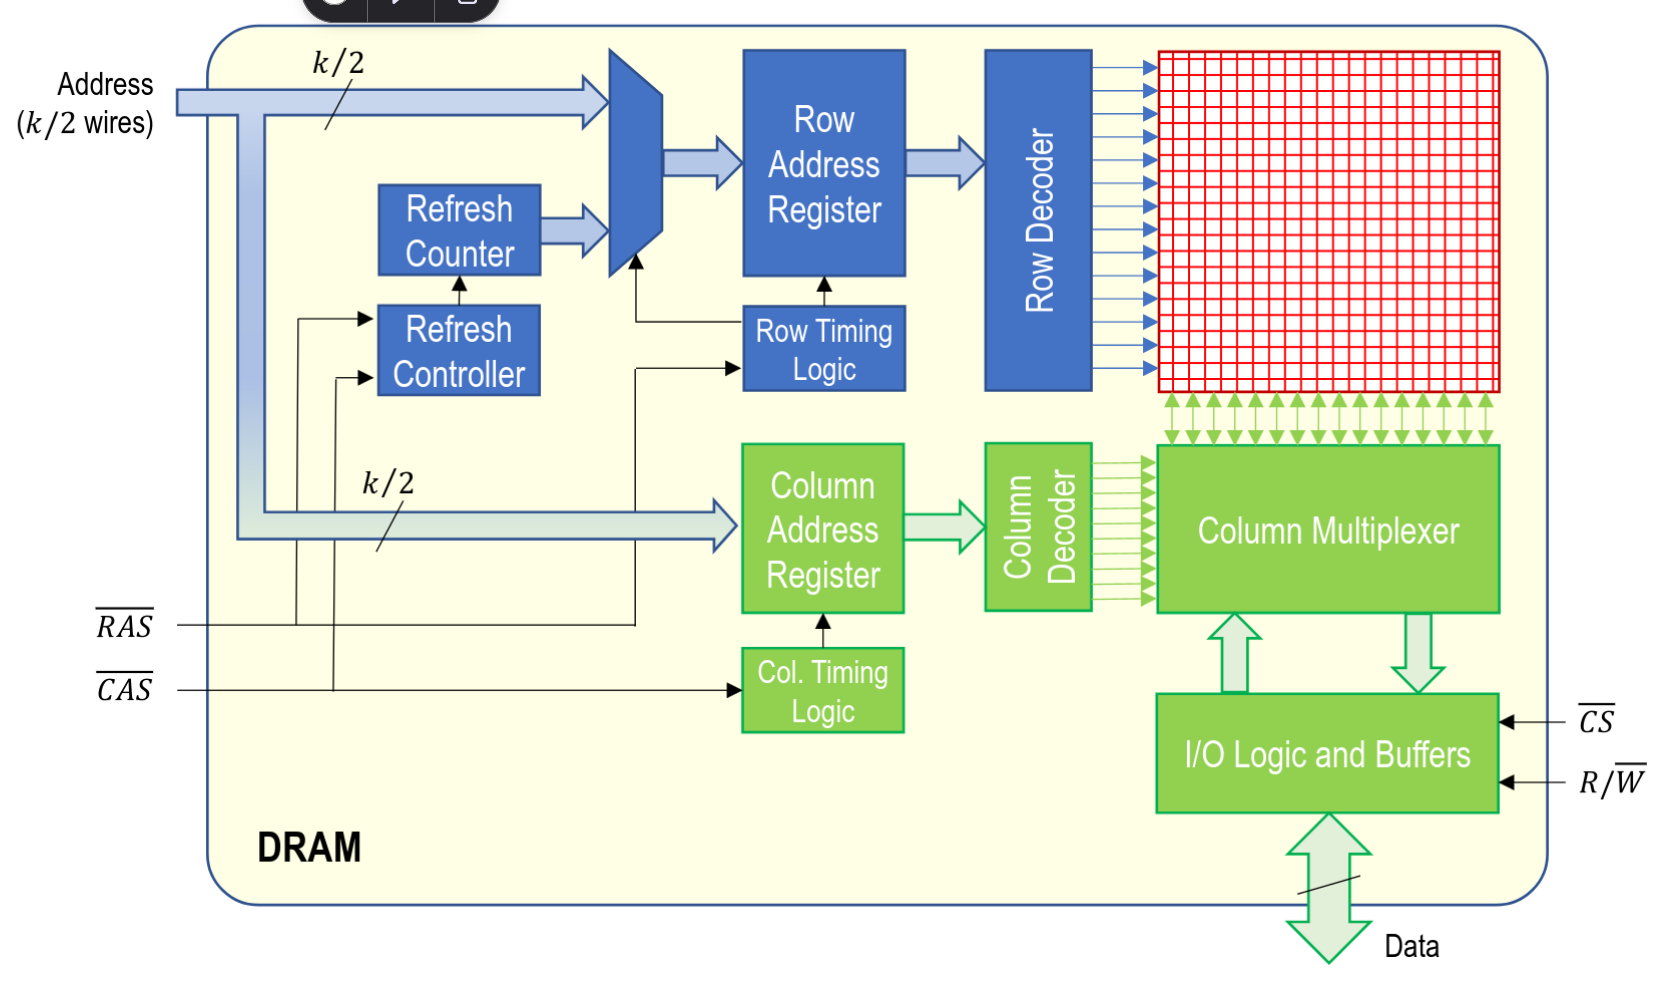
\includegraphics[scale=0.22]{../figures/dram_inter.png}
\end{center}

For the overall structure we see that we multiplex two halves of the address in time, using row and column registers.
This requires the additional control signals \textbf{RAS} (\textit{Row Address Strobe}) and \textbf{CAS} (\textit{Column Address Strobe}), usually active low.
\textit{Strobe} signals are signals used to notify the memory when an address is ready (column or row).

As for \textit{refreshes} (see the previous paragraph), we have that when a row is opened,
all data is refreshed.
Special circuits for automatic refresh are needed if refresh is automatic.
Refresh can also issued by a microprocessor (CAS before RAS).
Usually, when refreshes are issued by the microprocessor (or other external circuits), at least one read per each wordline has to be performed manually in a certain time period (the $T_{refresh}$ we calculated in the previous section).
Of course, as we saw, there is an \textit{overhead} due to refresh.

Let us now look at the timings for a simple read operations, to get an idea of the typical timing of the interface.

\begin{center}
	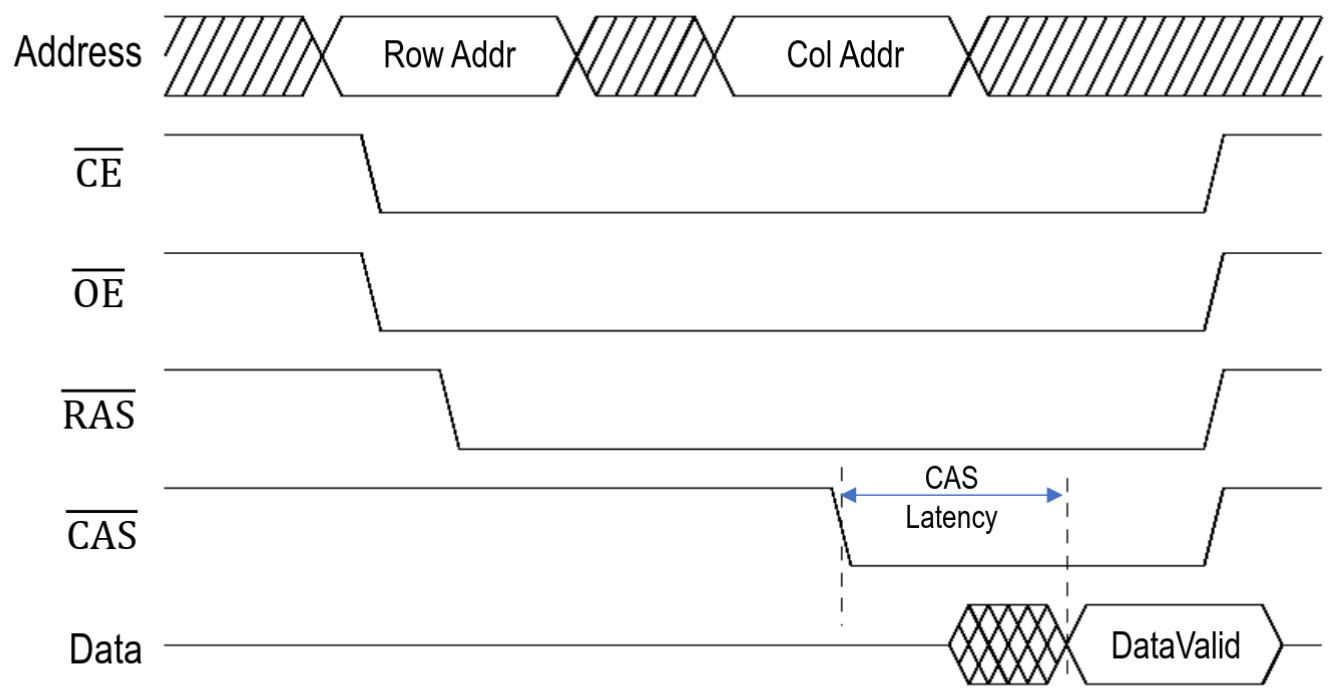
\includegraphics[scale=0.22]{../figures/norm_dram_time.png}
\end{center}

\begin{itemize}
	\item \textbf{Read operation} (\(\overline{\mathrm{CE}}=0\), \(\overline{\mathrm{WE}}=1\)):
	      \begin{itemize}
		      \item Present the Row Address (most significant bits) at the address pins and activate \(\overline{\mathrm{RAS}}\) (low) to latch it internally;
		      \item Present the Column Address (least significant bits) at the address pins and activate \(\overline{\mathrm{CAS}}\) (low) to latch it internally;
		      \item After a minimum delay, the output data is valid and stable.
	      \end{itemize}
\end{itemize}

\subsubsection{DRAM variations}

DRAM is relatively slow because reading data requires precharging the bit lines, selecting (opening) a row, and waiting for the sense amplifiers to detect the resulting voltage changes.
Because of this, some variations exist.
\begin{itemize}
	\item Since the row address is sufficient to open a row (or page), \textbf{Fast Page} Mode exploits the fact that all words in the same row are sensed, even those that are not explicitly read, and must also be rewritten. Once a row is open, other words within the same row can be accessed by specifying only the column address; these words need not be contiguous. To read another word in Fast Page Mode, a normal read operation is performed while keeping RAS active. CAS is then deactivated (set high), a new column address is presented at the address pins, and CAS is reactivated (set low) to latch the new column address internally. After a minimum delay, the new output data becomes valid and stable;

	\item \textit{Extended Data Out} (\textbf{EDO}) Mode is similar to Fast Page Mode, but with an additional register added at the output of the memory. The Column Address can change while keeping the data of the previous operation on the DataOut Bus.
	      This is not possible in Fast Page Mode, and the additional register implements a sort of small pipeline, increasing performance (we can change the column address while reading a word);

	\item \textit{Synchronous DRAM} (\textbf{SDRAM}): all operations synchronized on the active edge of a clock. This simplifies internal structure compared to asynchronous memories.
	      Simple circuits improve performance.
	      These RAMs allow for contiguous addresses, column sent only once. This is useful using caches;

	\item \textit{Double Data Rate} (\textbf{DDR}) is a variation on SDRAM. For contiguous data, the output is updated on both clock edges (rising and falling). For faster operation, we can use multiple clock edges, from multiple clocks out of phase.

	      There are different DDR DRAM variations:
	      \begin{itemize}
		      \item Normal applications: DDR, DDR2, DDR3, DDR4, ...
		      \item Low Power, for mobile applications: LPDDR1, LPDDR2, ...
		      \item High bandwidth, for graphic applications: GDDR2, GDDR3, GDDR4, GDDR5, ...
		      \item Special architectures such as RAMBus and eDRAM.
	      \end{itemize}

\end{itemize}

\end{document}
